\documentclass{amsart}
\usepackage[nosetup]{tony}
\usepackage{graphicx}

\title{6.867: Problem Set 1}
\date{September 29, 2016}

\begin{document}

%\begin{abstract}
%% #PLACEHOLDER
%MY ABSTRACT HERE summary summary
%\end{abstract}

\maketitle




% % % % % % % % % %
%    PROBLEM 1
% % % % % % % % % %

\section{Gradient Descent}

\subsection{Batch Gradient Descent}

We implemented a general-purpose batch gradient descent as described in Bishop 5.2.4, with user-specified objective function and gradient thereof, initial guess, step size, and termination criterion. % TODO elaborate on this?
We tested our implementation against two functions: a sign-reversed multivariate Gaussian with mean~$\mu$ and covariance matrix~$\Sigma$
\begin{equation}
f(x; \mu, \Sigma) = -\frac{1}{\sqrt{(2\pi)^n \det\Sigma}}\exp\left( -\frac12(x - \mu)^T \Sigma^{-1}(x - \mu) \right)
\end{equation}
and a quadratic bowl
\begin{equation}
f(x; A, b) = \frac{1}{2}x^T Ax - x^T b,
\end{equation}
where $A$ is positive-definite.

% TODO Do something with this
% For the Gaussian, we had $\mu = (10, 10)^T$, $\Sigma = \left(\begin{array}{cc}1000 & 0 \\0 & 1000\end{array}\right)$. For the quadratic bowl, we had $A = \left(\begin{array}{cc}10 & 5 \\5 & 10\end{array}\right)$ and $b = (400, 400)^T$.

% #PLACEHOLDER
% TODO
% present results of experiments
% "Discuss (and illustrate) the effect of the choice of starting guess, the step size, and the convergence criterion on the resulting solution, as well as how the norm of the gradient evolves through the iteration.

\subsection{Numerical Gradient Approximation}
\label{subsec:grad-approx}

Recall that our gradient descent procedure requires the user to specify both the objective function \emph{and} its gradient. With our examples, these gradients had simple analyic forms, but such is not the case for general objective functions. Therefore, as a check on the user-specified gradient (or as a substitute for a user-specified gradient), we implemented a gradient approximation routine.

Our procedure approximates the gradient of a general function~$f:\RR^d\to\RR$ at some given point~$x^*$ by approximating its partial derivatives as
\begin{equation}
\label{eq:grad-approx}
\f{\pa f}{\pa x_i}(x^*) \approx \f{f(x^* + \f12\eps\hat x_i) - f(x^* - \f12 \eps\hat x_i)}{\eps},
\end{equation}
where $\eps > 0$ is some user-supplied small difference step and where $\hat x_i$ is the unit vector in the $x_i$ direction. We compute this approximate partial derivative along each dimension of our domain and collect the values into our numerical gradient approximation. 

% #PLACEHOLDER
% TODO
% "Verify the gradient values on the functions you used in the question above by comparing the closed-form and numerical gradients at various points. Discuss the effect of changing the difference step (or "delta") on the accuracy of the gradient evaluation."

We note that decreasing the difference step increases the accuracy of the gradient evaluation, until round-off errors again decrease said accuracy around [todo].

\subsection{Stochastic Gradient Descent}

By design, batch gradient descent determines each update step by looking at the entire dataset and taking a gradient. This approach clearly becomes unfeasible with large datasets, and does not extend easily to online settings. For these reasons, we instead use stochastic gradient descent (SGD), in which we approximate the gradient as follows.

Suppose our objective function takes the form
\begin{equation}
J(\theta) = \sum_i J_i(\theta)
\end{equation}
where each $J_i$ is presumably a term corresponding to a single data point. Whereas the batch gradient descent update step takes a gradient over all $J$:
\begin{equation}
\theta_{t+1} = \theta_t - \eta \nabla J(\theta_t),
\end{equation}
the SGD update step has the form
\begin{equation} \theta_{t+1} = \theta_t - \eta_t \nabla J_i(\theta_t). \end{equation}

Note two key differences. We take $\nabla J_i$ as an approximation of $\nabla J$. More interestingly, our step size is now time-dependent. Because SGD is stochastic, it is unclear that SGD converges. But it can be shown that if we choose a learning rate schedule $\eta_t$ satisfying the Robbins-Monro conditions ($\sum_{t=1}^\infty \eta_t$ diverges and $\sum_{t=1}^\infty \eta_t^2$ converges), we get guaranteed convergence.

% #PLACEHOLDER
% TODO describe specific problem
% TODO talk about learning rate schedule and stopping criterion we chose for specific problem
% TODO part 1c

rem ipsum lorem ipsum lorem ipsum lorem ipsum lorem ipsum lorem ipsum lorem ipsum lorem ipsum lorem ipsum lorem ipsum lorem ipsum lorem ipsum lorem ipsum lorem ipsum lorem ipsum 



% % % % % % % % % %
%    PROBLEM 2
% % % % % % % % % %

\section{Linear Regression}

Before we proceed, recall that a linear basis function model for a dataset $(x^{(n)},y^{(n)})$ given a fixed set of basis functions $\phi_i$ is a regression model that tries to find weights~$w_i$ for which we approximately have
\[ y^{(n)} = w_0 + \sum_i w_i \phi_i(x^{(n)}). \]
In other words, we transform the independent variable $x$ by basis functions $\phi_i$, then perform linear regression with independent variables $\phi_i(x)$ and dependent variable~$y$.

We wrote a procedure for general linear basis function regression with user-specified data points and basis functions that found the maximum-likelihood weight vector analytically, via Bishop Equation 3.15, which we restate here:
\begin{equation}
\label{eq:max-likelihood-weights}
w = (\Phi^T\Phi)\inv\Phi^T Y
\end{equation}
where $Y$ is a vector of $y^{(n)}$ values from our dataset and $\Phi$ is the design matrix, given by
\begin{equation}
\Phi_{ij} = \phi_j(x^{(i)}).
\end{equation}

\subsection{Polynomial Basis Functions}

We tested our procedure by performing fits on a dataset of 11 points with polynomial basis functions up to some specified degree $M$. The dataset was generated by applying noise to the values produced by the function
\begin{equation}
y(x) = \cos(\pi x) + \cos(2\pi x).
\end{equation}
We plot the results of these fits for varying values of degree~$M$ in Figure~\ref{fig:2.1-polybasis}. Note the obvious underfitting and overfitting introduced by using models with excessively low or high degrees.


\begin{figure}[h] %  figure placement: here, top, bottom, or page
   \centering
   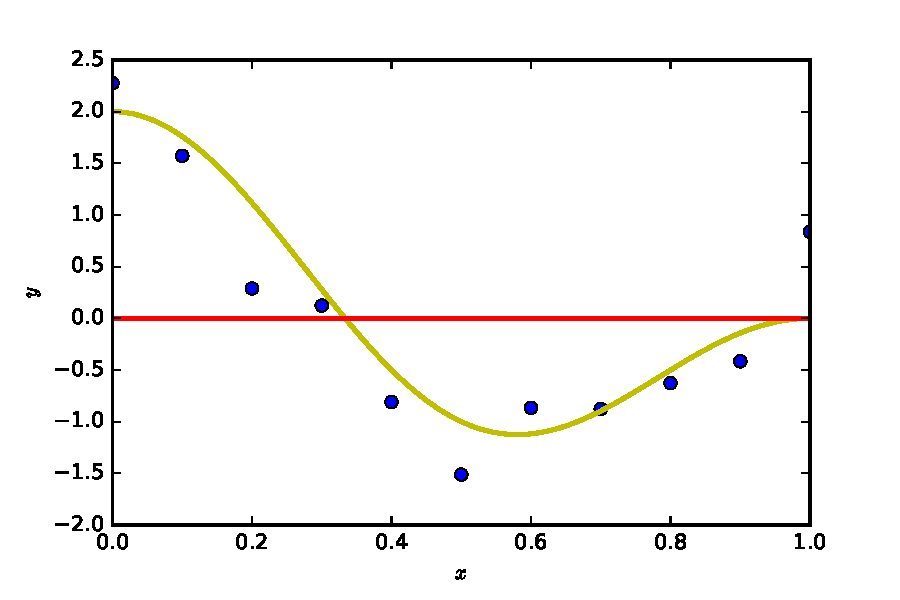
\includegraphics[width=2.25in]{img/2-1_degree0.pdf}  % $PLACEHOLDER
   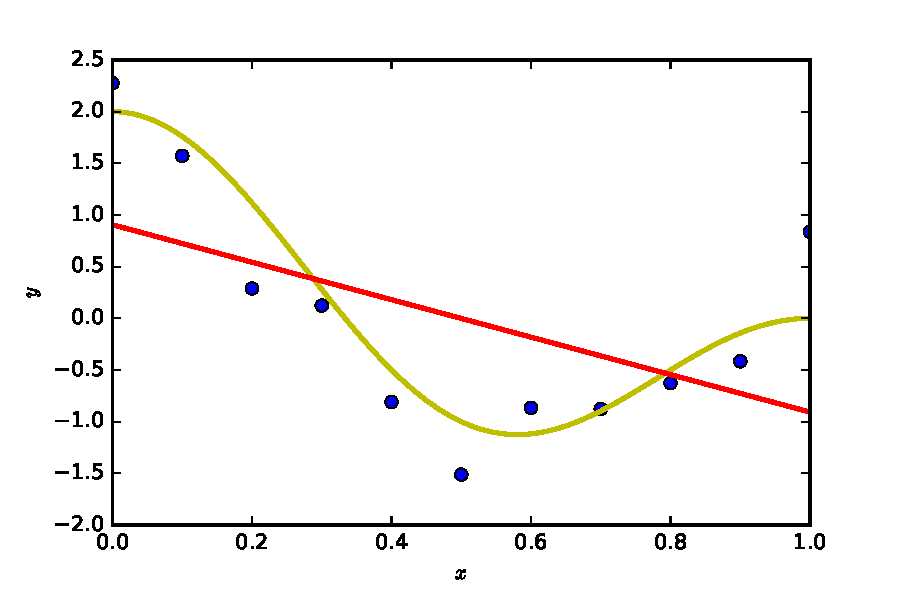
\includegraphics[width=2.25in]{img/2-1_degree1.pdf}  % $PLACEHOLDER
   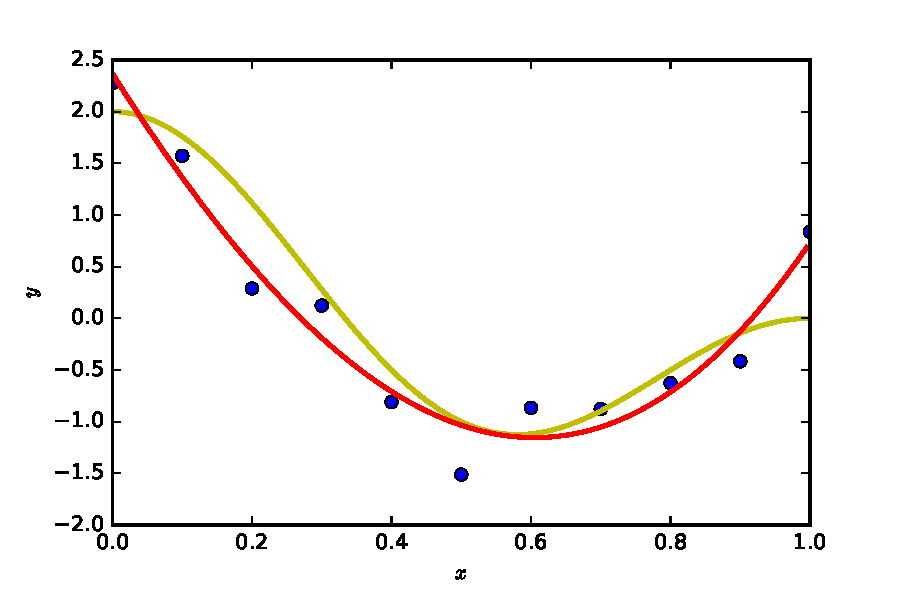
\includegraphics[width=2.25in]{img/2-1_degree3.pdf}  % $PLACEHOLDER
   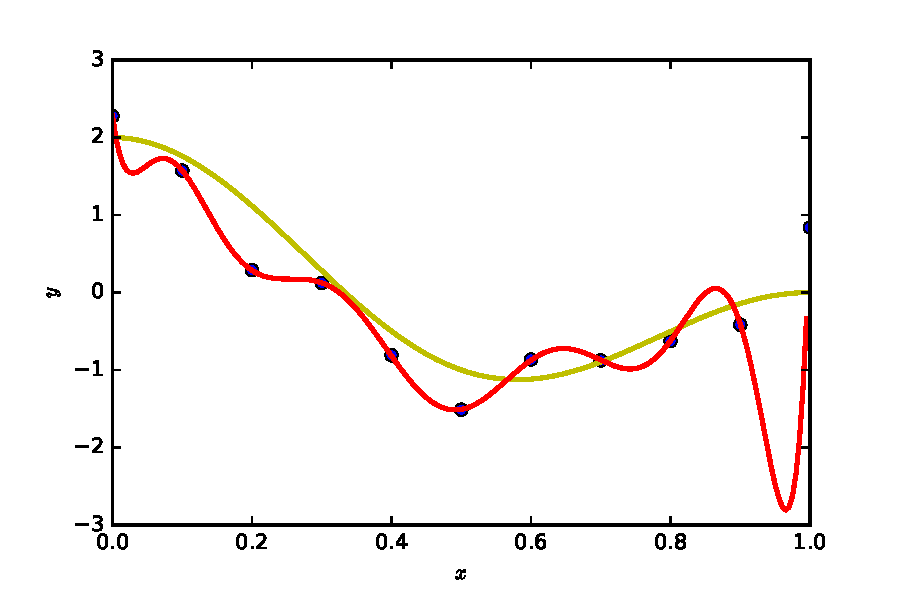
\includegraphics[width=2.25in]{img/2-1_degree10.pdf}  % $PLACEHOLDER
   \caption{Plots of our polynomial basis fits for degrees $M=0,1,3,10$. The degree ascends from top to bottom, and within each row, from left to right. The red curves are the polynomial fits; the yellow curve is the actual function used to generate the dataset, which is plotted in blue.}
   \label{fig:2.1-polybasis}
\end{figure}


\subsection{Regression by Gradient Descent}

Though there is a closed-form formula for the best-fit weight vector (Equation~\ref{eq:max-likelihood-weights}), we decided to verify our results from the previous section through gradient descent.

To this end, we considered the sum-of-squares error (SSE) for our problem:
\beq
J(w) = \f12 \sum_n \lt(y^{(n)} - \sum_j\phi_j(x^{(n)}) w_j\rt)^2 = \f12 (\Phi w - Y)^T(\Phi w - Y),
\eeq
which has gradient
\beq
\label{eq:sse-grad}
\nabla J(w) = \Phi^T(\Phi w - Y).
\eeq
Using our numeric gradient approximation from section~\ref{subsec:grad-approx} (Equation~\ref{eq:grad-approx}), we verified the correctness of Equation~\ref{eq:sse-grad}.

We proceeded to estimate the maximmum-likelihood weight vector $w$ (Equation~\ref{eq:max-likelihood-weights}), which minimizes squared sum error, using batch gradient descent.
For small degree fits, the results agreed strongly with the closed-form solution.
However, for higher degrees, the discrepancies between our maximum-likelihood fits and our gradient-descent estimate fits grew progressively larger (Figure~\ref{fig:bgd-poly-fits}).

Interestingly, the gradient descent fits did not overfit nearly as much as the maximum-likelihood fits at high degree.
We conjecture that this behavior arises because we initialize our weight vectors at 0, ``regularizing" our fits in a sense.
Moreover, our gradient descent procedure terminates when the objective function changes between gradient descent iterations drops below a certain threshold, which we can think of as a form of early stopping.

\begin{figure}[h]
   \centering
   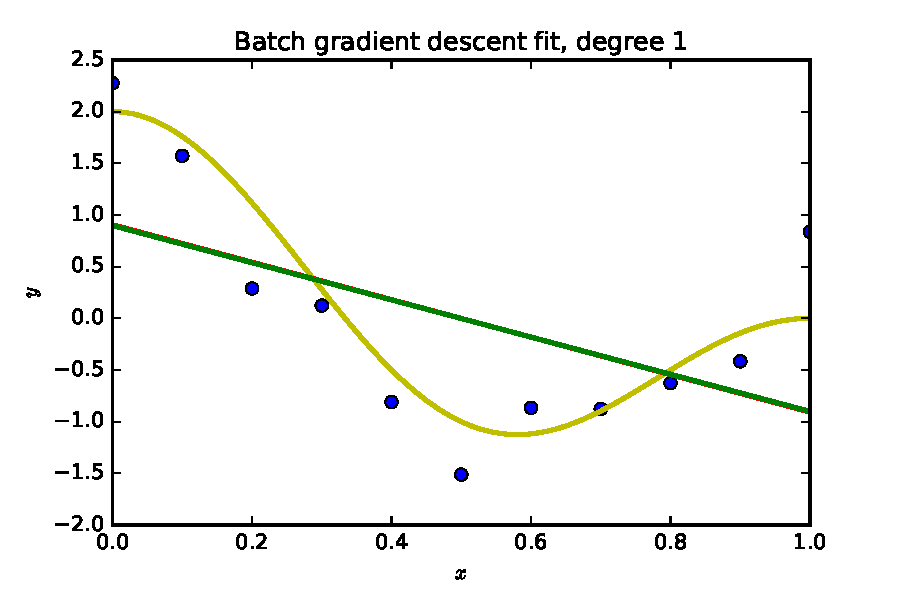
\includegraphics[width=2.25in]{img/2-3_bgd_fit_degree1.pdf}
   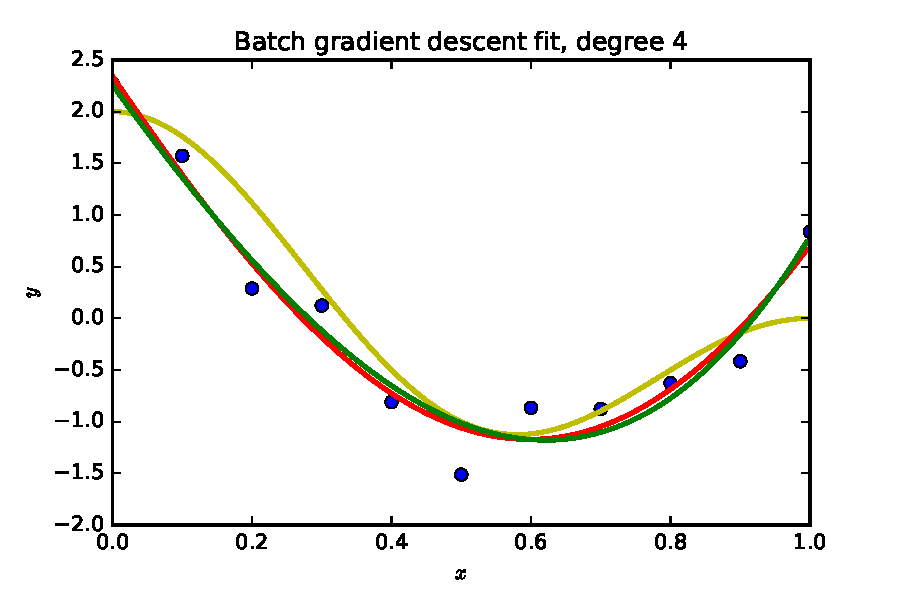
\includegraphics[width=2.25in]{img/2-3_bgd_fit_degree4.pdf}
   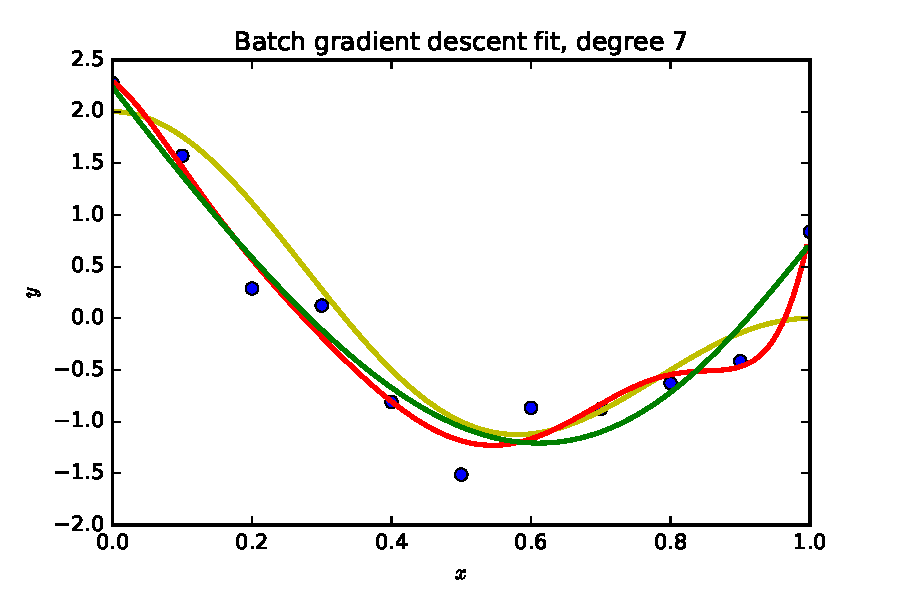
\includegraphics[width=2.25in]{img/2-3_bgd_fit_degree7.pdf}
   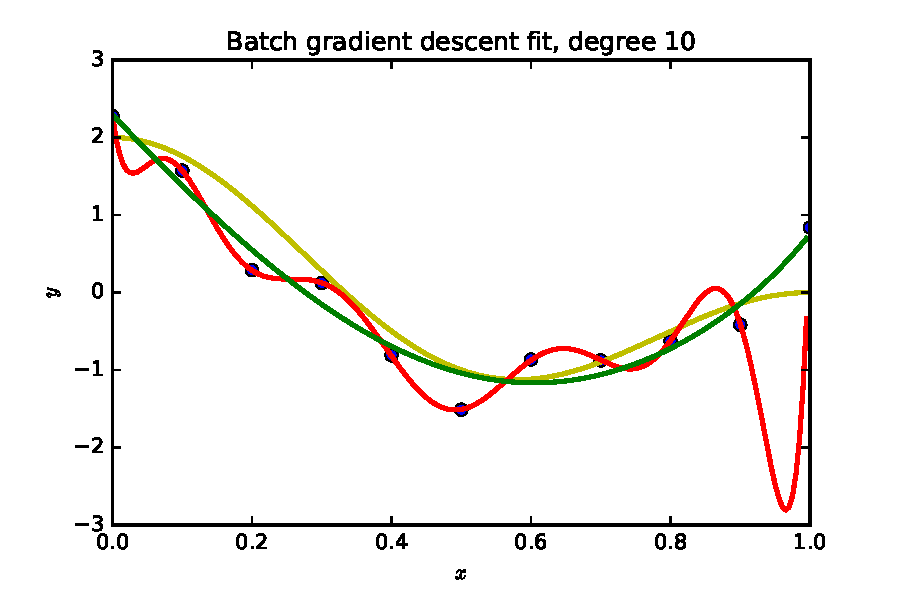
\includegraphics[width=2.25in]{img/2-3_bgd_fit_degree10.pdf}
   \caption{Polynomial fits by batch gradient descent of various degrees (green) of the dataset (blue) generated from a sum of cosines (yellow).
   The fits agree perfectly with the maximum-likelihood fits (red) at low degrees, but differ increasingly for higher degrees.
   }
   \label{fig:bgd-poly-fits}
\end{figure}

% 2b/c

% Use batch gradient descent on the SSE function on some values of M.
% Describe your experience with initial guesses, step sizes and convergence thresholds.
% Compare with using SGD on the same data.
% Explain your results in terms of the properties of the function being optimized and the properties of the algorithms.

% #PLACEHOLDER

rem ipsum lorem ipsum lorem ipsum l ipsum lorem ipsum lorem ipsum lorem ipsum lorem ipsum lorem ipsum lorem ipsu

m lorem ipsum lorem ipsum lorem ipsorem ipsum lorem ipsum lorem ipsum lorem ipsum lorem 

\subsection{Cosine Basis Functions}

ipsum lorem ipsum lorem ipsum loremum lorem ipsum lorem ipsum lorem ipsum lor

em ipsum lorem ipsum lorem ipsum lorem ipsum lorem ipsum lorem ipsum lorem ipsum




% % % % % % % % % %
%    PROBLEM 3
% % % % % % % % % %

\section{Ridge Regression}

% #PLACEHOLDER

rem ipsum lorem ipsum lorem ipsum lorem ipsum lorem ipsum lorem ipsum lorem ipsum lorem ipsum lorem ipsum lorem ipsum lorem ipsum lorem ipsum lorem ipsum lorem ipsum lorem ipsum lorem ipsum lorem ipsum l

orem ipsum lorem ipsum lorem ipsum lorem ipsum lorem ipsum lorem ipsum lorem ipsum lorem ipsum lorem ipsum lorem ipsum lorem ipsum lorem ipsum lorem ipsum




% % % % % % % % % %
%    PROBLEM 4
% % % % % % % % % %

\section{Sparsification with LASSO}

% #PLACEHOLDER
lorem ipsum lorem ipsum lorem ip

sum lorem ipsum lorem ipsum lorem ipsum lorem ipsum lorem ipsum lorem ipsum lorem ipsum lorem ipsum lorem ipsum lorem ipsum lorem ipsum lorem ipsum lorem ipsum lorem ipsum lorem ip

sum lorem ipsum lorem ipsum lorem ipsum lorem ipsum lorem ipsum lorem ipsum lorem ipsum lorem ipsum lo

lorem ipsum lorem ipsum lorem ipsum lorem ipsum lorem ipsum lorem ipsum lorem ipsum lorem ipsum lorem ipsum lorem ipsum lorem ipsum lorem ipsum lorem ipsum lorem ipsum lorem ipsum lorem ipsum lorem ipsum lorem ipsum lore

m ipsum lorem ipsum lorem ipsum lorem ipsum lorem ipsum lorem ipsum lorem ipsum lorem ipsum lorem ipsum lorem 


 lorem ipsum lorem ipsum lorem ipsum lorem ipsum lorem ipsum lorem ipsum lorem ipsum lorem ip
 sum lorem ipsum lorem ipsum lorem ipsum lorem ipsum lorem ipsum lorem ipsum lorem ipsum l
 
 orem ipsum lorem ipsum lorem ipsum lorem ipsum lorem ipsum lorem ipsum lorem ipsum lorem i
 psum lorem ipsum lorem ipsum lorem ipsum lorem ipsum lorem ipsum  

\end{document}
